\newpage
\pagestyle{fancy}
\fancyhead[RO]{\nouppercase{\textbf{Κεφάλαιο \ref{Ch:intro}} $|$ \textit{\nameref{Ch:intro}}}}
\fancyhead[LE]{\textit{\nameref{Ch:intro}} $|$ \nouppercase{\textbf{Κεφάλαιο \ref{Ch:intro}}}}
\setcounter{page}{1}
\setcounter{chapter}{0}

\pagenumbering{arabic}

\chapter{Εισαγωγή}
\label{Ch:intro}
%\lipsum\lipsum\lipsum

\section{Σημασία του Αντισεισμικού Σχεδιασμού Υπογείων Έργων}
% Πρώτα μια παραγραφούλα γι την σημασία των σηράγγων, κρίσιμη υποδομή και τέτοια. Μετά γιατί ο κόσμος αναπτύσσεται και γίνεται πιο ευαίσθητος στην αλλαγή, πως ο σχεδιασμός πρέπει να περιλαμβάνει την πρόβλεψη και την ανθεκτικότητα. Έτσι πως η ανάλυση έιναι απαραίτητη για βιώσιμο σχεδιασμό ή κάτι τέτοιο. Θα το δω το πρωί τώρα, γράφω και κλειστά αυτή την στιγμή, και έτσι πιστεύω ότι μπορώ να γεμίσω μισή σελιδούλα με αυτό.

Οι μετακινήσεις αποτελούν αναπόσπαστο κομμάτι όλων των κοινωνιών, εξελισόμενες πάντοτε παράλληλα με τους πολιτισμούς. Στην σύγχρονη εποχή, όπου ο χώρος δομείται με γεωμετρική πρόοδο τόσο αυξάνεται η ανάγκη των μετακινήσεων, όσο και παρεμποδίζεται η εκτέλεση των. Επομένως, η εκμετάλλευση του χώρου σε μία τρίτη διάσταση, εν προκειμένω εντός της Γης, καταλύει την δημιουργία λύσεων των αστικών μετακινήσεων με την κατασκευή μητροπολιτικών σηράγγων, γνωστών και ως μετρό.

Οι πληθωρικώς ανεπτυγμένες υποδομές όμως, παρουσιάζουν αυξημένη ευαισθησία στις εξωτερικές παρεμβολές και επιδράσεις καθώς ο παρεμποδισμός, σε μικρό βαθμό, μίας κρίσιμης υπηρεσίας μπορεί να έχει τεράστιες συνέπειες σε τέτοια περιβάλλοντα.

Μάλιστα, τέτοια φαινόμενα έχουν συσσωρευτικό χαρακτήρα, όπως είναι, ο ενδιαφερόμενος σε τούτη την εργασία, σεισμός. Για παράδειγμα, η λειτουργική αστοχία μίας γέφυρας λόγω διαφορικής καθίζησης των βάθρων της μετά από σεισμό, η ρευστοποίηση ενός οδικού επιχώματος ή τα συντρίμμια μίας κατασκευής σε έναν δρόμο πέρα από μία αυτοτελή καταστροφή, κωλύουν την εκκένωση των κατοίκων και την μεταφορά οχημάτων εκτάκτου ανάγκης παράγοντας έτσι πρόσθετη ζημία.

Οι αναφερόμενες, και άλλες παρόμοιες, συνθήκες είναι που καθιστούν τις σύγχρονες υποδομές ιδιαίτερα ευαίσθητες στα έντονα φυσικά φαινόμενα και καθιερώνοντας τις σεισμικές δράσεις, ως βασική απειλή για όλα τα έργα υποδομής. Έτσι οαντισεισμικός σχεδιασμός των έργων αποτελεί βασικό τμήμα κάθε μελέτης σε περιοχές ενεργού σεισμικότητας. Η ίδια προσοχή όμως, δεν λαμβάνεται πάντοτε για τα υπόγεια έργα.

Οι υπόγειες κατασκευές -και ιδιαιτέρως οι σήραγγες- χαρακτηρίζονται από τον εγκιβωτισμό τους στο έδαφος. Αυτό σημαίνει ότι οι μετατοπίσεις του εδάφους ορίζουν τις παραμορφώσεις των σηράγγων και όχι το αντίθετο. Στην πράξη, οι σήραγγες δεν επιφορτίζονται από αδρανειακές δνάμεις, όπως είναι το αναμενόμενο σε επιφανειακές κατασκευές, αλλά από κινηματικές δράσεις. Αυτό το φαινόμενα, τυπικά, ένισχύεται με την αύξηση του βάθους, και θα φανεί και στην συνέχεια ότι οι δράσεις των ταχυτήτων είναι βασική παράμετρος για τις βαθιές σήραγγες.

Επομένως, ο αντισεισμικός σχεδιασμός των σηράγγων συχνά αγνοείται, με γνώμονα ότι ο κίνδυνος κατάρρευσης παρουσιάζεται αποκλειστικά σε ρηχές σήραγγες κατασκευασμένες σε μαλακές αποθέσεις. Η ιστορία όμως, έχει αποδείξει το αντίθετο. Με σήραγγες και σταθμούς, οι οποίοι υπέστησαν με μεγάλες καταστροφές ή και καταρρεύσεις μετά από σεισμικές ακολουθίες. Τέτοια παραδείγματα είναι η κατάρρευση του σταθμού Νταϊκαϊ στην Ιαπωνία, στον σεισμό Χιόογκοκεν-Νάμπου το 1995, η αστοχίες στην σήραγγα Λόνγξι του σεισμού της Γουέντσουαν το 2008 ή και οι πολύ πρόσφατες καταρρεύσεις στις πολλαπλές οδικές σήραγγες της Τουρκίας μετά την Τουρκο-Συριακή σεισμική ακολουθία του 2008.

Επομένως, η μελέτη της σεισμικής τρωτότητας σηράγγων δικαιολογείται στην πράξη, και πρέπει να αποτελεί μία σταθερή τακτική στον σχεδιασμό και την διαχείριση τόσο κρίσιμων υπόγειων υποδομών.

\section{Ορισμοί}
\subsection{Διακινδύνευση}
\label{Sbsec:Haz}
Η σεισμική διακινδύνευση (Risk) ορίζεται ως η αναμονέμενες ζημίες ή απώλειες σε κάποια περιοχή μελέτης για δεδομένη σεισμική δραστηριότητα.

Η σεισμική δραστηριότητα καθορίζεται από την ανάλυση επικινδυνότητας (Hazard), όπου προβλέπεται η πιθανότητα στον χρόνο να παρουσιαστεί ένα μέγθος σεισμικής έντασης.

Οι ζημιές στην θέση μελέτης, καθορίζονται από τις δύο παραμέτρους της τρωτότητας (Vulnerability) και της έκθεσης (Exposure). Η σεισμική τρωτότητα, εκφράζει την πιθανότητα παρουσίας βλαβών, δεδομένου ενός μεγέθους έντασης, εκφράζει έτσι την αναμενόμενη απώλεια για ένα συγκεκριμένο συμβάν. Η έκθεση είναι μία παράμετρος που εκφράζει καθαρά την αξία των κατασκευών, μεταβάλλοντας το μέγεθος της διακίνδευσης αναλόγως την σπουδαιότητα της κατασκευής. \parencite{Pitilakis}

\subsection{Ευαισθησία}
Η ευαισθησία (Vulnerability) πρόκειται για ένα μέγεθος συγγενές της τρωτότητας. Αντί όμως να αφορά την πιθανότητα εκδήλωση μίας κατάστασης για ένα δεδομένο μέγεθος έντασης, παρουσιάζει το αναμενόμενο κόστος σε κάθε αντίστοιχο μέγεθος έντασης.

\subsection{Μέγεθος Έντασης}
Μέγεθος Έντασης (Intensity Measure, IM), ονομάζεται μία παράμετρος κατηγοροιοποίησης της σεισμικής δράσης και συσχέτισης με την επικινδυνότητα.

Συνήθως λαμβάνεται ως η μέγιστη επιτάχυνση, ταχύτητα ή μετατόπιση ($PGA$, $PGV$, $PGD$), αλλά μπορεί να λάβει διάφορες τιμές, όπως η ένταση Arias ($I_A$), ο λόγος της μέγιστης κατακόρυφης επιτάχυνσης προς την οριζόντια ($FR1$) ή την διατηρούμενη μέγιστη επιτάχυνση ή ταχύτητα ($SMA$, $SMV$).

Στην παρούσα εργασία θα χρησιμοποιηθούν ως μεγέθη έντασης οι $PGA$ και $PGV$ όπως θα αναπτυχθεί στην σχετική ενότητα \parencite{Huang}.

\subsection{Παράμετρος Μηχανικής Ικανότητας}
Παράμετρος μηχανικής ικανότητας (Engineering Demand Parameter, EDP), ονομάζεται ένα μέγεθος καταπόνησης της κατασκευής, το οποίο μπορεί να χρησιμοποιηθεί για τον χαρακτηρισμό τωνο ριακών καταστάσεων λειτουργίας.

Οι τιμές EDP αποτελούν αποκρίσεις της μελετούμενης κατασκευής για σεισιμκές αναλύσεις, και συνήθως λαμβάνονται ως κάποιο μέγεθος τάσης ή παραμόρφωσης. Αυτό το μέγεθος πρέπει να επιλέγεται με τέτοιον τρόπο έτσι ώστε να εκφράζεται βέλτιστα την εξεταζόμενη αστοχία.

Για παράδειγμα έτοιες τιμές μπορεί να είναι η σχετική μετατόπιση ορόφων ενός κτηρίου ή η διαφορική καθίζηση μεταξύ των πελμάτων αυτού και άλλα.

Στην παρούσα εργασία, επιλέγονται ως EDPs για την παραγωγή ξεχωριστών καμπυλών τρωτότητας η ανηγμένη διαμετρική παραμόρφωση της κάθε σήραγγας και η ανηγμένη ροπή της εκάστοτε διατομής. Η ροπή είναι μία συνήθης EDP που χρησιμοποιείται σε αντίστοιχες μελέτες, επομένως η σύγκριση είναι εύκολη ενώ η διαμετρική παραμόρφωση 

\begin{figure}[ht]
	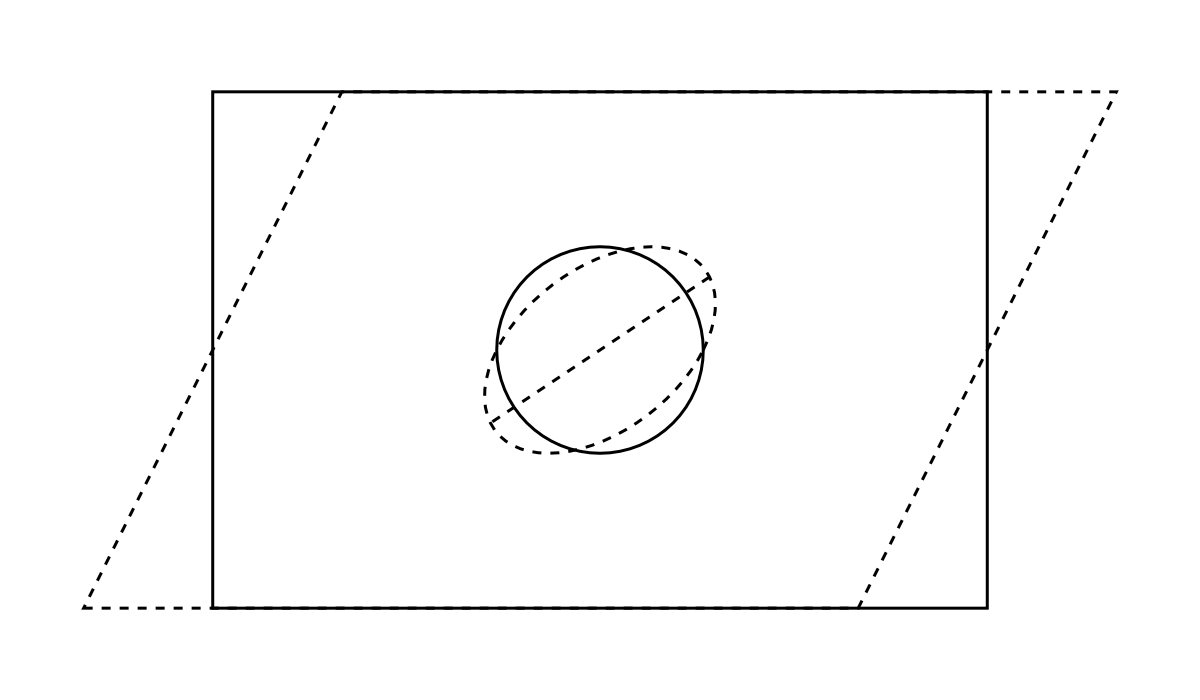
\includegraphics[width=0.9\linewidth]{figures/intro/deflection-example.png}
	\label{fig:defl}
	\caption{Διατμητική Παραμόρφωση Σηράγγων}
\end{figure}

Η ανηγμένη ροπή χρησιμοποιείται ευρεύως ως EDP σε κατασκευές, καθώς είναι εύκολο να συσχετιστεί σε σχέση με την φέρουσα ικανότητα μίας κατασκευής, εφόσον είναι γνωστή η γεωμετρία μίας διατομής και οι ποιότητες των υλικών.

Η διαμετρική παραμόρφωση πρόκειται για τιμή που χρησιμοποιείται σε κυκλικές διατομές που υπόκεινται σε διατμητικές παραμορφώσεις. Ο λόγος είναι ότι η διατμητική παραμόρφωση προκαλεί μία οβαλοποίηση στις κυκλικές διατομές, η οποία παραμόρφωση ελαττώνει έντονα την δυσκαμψία της ενώ είναι εύκολη η μέτρηση της μεταβολής της διαμέτρου.

Καθώς τα κύρια σεισμικά κύματα που έπηρεάζουν την σήραγγα, και αυτά που μελετώνται, είναι τα διατμητικά, όπως αναφέρεται αργότερα και στην Υποενότητα \ref{sbs:Waves}, καθίσταται σαφές το γεγονός ότι η σήραγγα υπόκειται σε διατμητικές παραμορφώσεις.

Στο Σχήμα \ref{fig:defl} απεικονίζεται ο τρόπος που παραμορφώνεται η σήραγγα όταν μεταδίδονται διατμητικά κύματα μέσα στο έδαφος. Με συνεχείς γραμμές παρουσιάζεται το έδαφος και η σήραγγα πριν παραμορφωθεί, ενώ με διακεκομμένη γραμμή παρουσιάζονται μετά από την ένταση. Παρατηρείται σαφώς το φαινόμενο οβαλοποίησης, όπου η σήραγγα παραμορφώνεται σε σχήμα έλλειψης. Η μέγιστη βράχυνση ή επιμήκυνση της διαμέτρου της σήραγγας είναι που δίνει την διαμετρική παραμόρφωση, ενώ μπορεί να παρατηρηθεί πως αυτή η παραμόρφωση εμφανίζεται στους άξονες $\pm 45^o$.


\subsection{Οριακές Καταστάσεις Λειτουργίας}
Ως οριακή καταστάση λειτουργίας (Limit States), ορίζεται η κατάσταση στην οποία βρίσκεται μία κατασκευή, δεδομένου ότι έχει ξεπεράσει ένα ορισμένο μέγεθος μίας EDP.

Ιδανικά οι οριακές καταστάσεις λειτουργίας πρέπει να ορίζονται με μεγάλη ακρίβεια και καθαρά ποσοτικά κριτήρια έτσι ώστε να αποφεύγεται η υποκειμενική ερμηνεία και η ανάγκη στις ερμηνείες ειδικών \parencite{Porter}. Δυστυχώς όμως, λόγω της περιορισμένης προσοχής που έχουν λάβει τα μελετούμενα φαινόμενα, στην συγκεκριμένη εργασίας λαμβάνονται ως οριακές καταστάσεις ολοκληρωτικής κατάρρευσης, εκτεταμένης καταστροφής και αντιστρέψιμης ζημιάς, και συσχετίζονται με την EDP σύμφωνα με τις γνωμοδοτήσεις ειδικών \parencite{TsinidisLS}.

\subsection{Πιθανοτική Ανάλυση}

Όσων αφορά της σεισμική ανάλυση των σηράγγων, η διαίσθση του μηχανικού σε σχέση με τα συνήθη ζητήματα οδηγεί στην σκέψη ότι  πρεπει να εκτιμηθεί μία μέγιστη πιθανή  τιμή επιτάχυνσης, που δύναται να ασκηθεί σε μία περιοχή, να πολλαπλασιαστεί με κάποιον συντελεστή σχεδιασμού και έπειτα να διαστασιολογηθεί η κατασκευή σύμφωνα με αυτή την τιμή. Η συγκεκριμένη μεθοδολογία χαρακτηρίζεται ως αιτιοκρατική μέθοδος (Epistemic Method) και η πράξη έχει δείξει ότι ένα χωροχρονικό φαινόμενο όπως ο σεισμός, δεν γίνεται να αναλυθεί ως κάποια "οριακή" κατάσταση, αλλά εμπεριέχει εν γένει αβεβαιότητες \parencite{Pitilakis}.

Έτσι, αναπτύχθηκε στα μέσα του προηγούμενου αιώνα μία πιθανοτική (Aleatory ή Probabilistic) μεθοδολογία που να βασίζεται ακριβώς σε αυτές τις αβεβαιότητες. Αυτή η μεθοδολογία ονομάζεται Probabilistic Seismic Hazard Analysis (PSHA) και εκφράζει, ότι κάθε σεισμική πηγή έχει μία πιθανοτική κατανομή η οποία ορίζει τα σεισμικά γεγονότα της. Έτσι, αντί να υπολογιστεί απ' ευθείας ένα μέγιστο μέγεθος σχεδιασμού, μπορεί να οριστεί μία τιμή για κάποια αποδεκτή πιθανότητα. Στους σύγχρονους κανονισμούς, αυτή η πιθανότητα εκφράζεται συνήθως ως ο αριθμός των σεισμικών γεγονότων ενός μεγέθους σε ορισμένο χρονικό πλαίσιο.

Αυτή η μεθοδολογία ακολουθείται και στην συγκεκριμένη εργασία έτσι ώστε να εκτιμηθεί η επικινδυνότητα του έργου, όπως αυτή ορίστηκε στην Υποενότητα \ref{Sbsec:Haz}.

\section{Παραδείγματα Αστοχιών}
\subsection{Σταθμός Νταϊκαϊ}
Μία από τις χαρακτηριστικότερες αστοχίες υπογείων έργων, είναι η πρώτη κατάρρεση σταθμού μετρό στο Κόμπε της Ιαπωνίας. Στις 17 Ιανουαρίου του έτους 1995, συνέβη ο σεισμός του Χιόγκοκεν-Νάνμπου, ένας από τους ισχυρότερους σεισμούς της σύγχρονης ιστορίας έντασης JMA 7 (MM 10) όπως εκδηλώνεται από τα καταστροφικά αποτελέσματα του.

Πριν από την κατάρρευση του σταθμού, η επιρροή του σεισμού σε υπόγειες κατασκευές είχε μελετηθεί, αλλά κυρίως για σωληνώσεις που είναι ιδιαίτερα ευαίσθητες στην παραμόρφωση του εδάφους. Μέχρι εκείνο το σημείο θεωρούνταν ότι οι υπόγειες κατασκευές είναι ιδιαίτερα ανθεκτικές στον σεισμό και οι συνθήκες αστοχίας έφεραν άλλες μεθοδολογίες στο προσκήνιο

Το έργο αφορά έναν επιμήκη σταθμό, με μήκος $120m$, πλάτος $17m$ και εξωτερικό ύψος $7.17m$ στις πλατφόρμες. Η κατασκευή χαρακτηρίστηκε σε τρεις ζώνες Α, Β και Γ περιγράφοντας την νοτιοδυτική πλατφόρμα, τον βασικό διώροφο όγκο με τα εκδοτήρια και την είσοδο και την βορειανατολική πλατφόρμα αντίστοιχα. Οι σημαντικότερες ζημιές και η κατάρρεση, συνέβησαν στην ζώνη Α, όπου δομικά περιγράφεται από δύο πλευρικούς τοίχους και μία σειρά από κεντρικά υποστυλώματα.

Στην αυτοψία που πραγματοποιήθηκε έναν χρόνο μετά την κατάρρευση, διαπιστώθηκε ότι η επιδραστικότερη διέγερση ασκήθηκε κατά το πλάτος του σταθμού, ξεπερνώντας την διατμητική δομική επάρκεια των υποστυλωμάτων και οδηγώντας τα σε μεγάλες διατμητικές παραμορφώσεις. Έπειτα, το βάρος της πλάκας οροφής (που ασκείται πλέον έκκεντρα) οδηγεί στην ανάπτυξη έντονων φαινομένων $P-\Delta$ μέχρι τα υποστυλώματα να καταρρεύσουν πλήρως. Η κατάρρευση των υποστυλωμάτων οδηγεί στην υποχώρηση της πλάκας και σε επιφανειακές καθιζήσεις που φτάνουν έως τα $2m$.

Στα πλαίσια της ίδιας εργασίας έγινε και η εκτίμηση του μηχανισμού άσκησης της οριζόντιας φόρτισης. Η υπόθεση των ερευνητών κατέληξε ότι ήταν σχετική παραμόρφωση της πλάκας βάσης με την πλάκα οροφής που οδήγησε στην ανάπτυξη υψηλών διατμητικών δυνάμεων, και όχι η άσκηση πλευρικών ωθήσεων \parencite{Ida}.

Ο γράφων θεωρεί το γεγονός ότι οι υπόγειες κατασκευές επηρεάζονται από τους σεισμούς, καθώς και τον μηχανισμό που καθορίζει αυτή την επιρροή, τα σημαντικότερα συμπεράσματα της μελέτης και σε μικρότερο βαθμό τον τρόπο αστοχίας. Εξάλλου, ένας δομοστατικός μηχανικός σίγουρα θα παρατηρούσε ότι η ζώνη Β παρουσίασε διατμητικές ρωγμές Χ \parencite{Karajohn}, σε αντίθεση με κατάρρευση υποστυλωμάτων. Μία τέτοια αστοχία θυμίζει μάλλον την λειτουργία των διατμητικών τοίχων σε σύγχρονες αντισεισμικές κατασκευές. Έτσι, ενδέχεται το μεγαλύτερο μέρος των αστοχιών να είχε αποφευχθεί εάν οι ζώνες Α και Β είχαν σχεδιασεί με πυρήνα και τοιχεία. 


\subsection{Σήραγγα Λόνγκξι}
Στο Γουέτσουαν της Κίνας, βρίσκεται η ορεινή οδική σήραγγα Λόνγκξι. Στις 12 του Μάη του έτους 2008, και σε επικεντρική απόσταση $2km$ η πρώτη εκτόνωση από την δεύτερη πιο καταστροφική σεισμική ακολουθία της Κίνας πραγματοποιήθηκε. Ο σεισμός είχε ως αποτέλεσμα την κατάρρευση του ανατολικότερου στομίου της σήραγγας, εκτεταμένες ζημιές κατά μήκος της και την ολοκληρωτική κατάρρευση σε ένα σημείο. Ακόμα, η αριθμητική μελέτη της αστοχίας, έδειξε ότι η συνισταμένη επίδραση τόσο της εγκάρσιας όσο και της διαμήκους διέγερσης, έχει σημαντική επιρροή στα αποτελέσματα και εμφανίζεται στις τρισδιάστατες αναλύσεις \parencite{Yu}. Η παρούσα μελέτη περιορίζεται σε δισδιάστατες αναλύσεις, αγνοώντας πλήρως την διαμήκη διέγερση.

Η σημασία της συγκεκριμένης αστοχίας, πηγάζει από το γεγονός ότι η σήραγγα τέμενται από ανάστροφο ρήγμα, το οποίο και ενεργοποιήθηκε με την σεισμική διέγερση, οδηγώντας σε ολοκληρωτική κατάρρευση το σημείο τομής. Ακόμα, η επικεντρική απόσταση φαίνεται να έχει μικρή επιρροή στο αποτέλεσμα, καθώς το ρήγμα βρίσκεται αρκετά μακρύτερα του επικέντρου σε σχέση με το δυτικό στόμιο, αλλά το πρώτο έχει πτωχότερους γεωλογικούς σχηματισμούς σε σχέση με το δεύτερο.

Σε σχέση με το μετρό Θεσσαλονίκης, η αναφορέμονη περίπτωση παρουσιάζει μεγάλο ενδιαφέρον καθώς αμφότερες οι σήραγγες τέμνουν από ένα ενεργό ρήγμα. Το μετρό της Θεσσαλονίκης συναντάει ένα κοντά στον σταθμό Βούλγαρη, και οι σήραγγες στο σημείο έχουν σχεδιαστεί ειδικά ώστε να λαμβάνουν υψηλές παραμορφώσεις εξαιτίας σεισμικών φαινομένων \parencite{Gavrielatou}. (Δεν έχω πρόσβαση σε αυτή την αναφορά, υπάρχει κάπου ή φτάνει;)

\subsection{Σήραγγες Καχραμάνμαρας}
Στην πιο πρόσφατη ιστορία, στις 6 Φεβρουαρίου 2023, στην Τουρκία, πραγματοποιήθηκε μία πολύ ισχυρή σεισμική ακολουθία που είχε ως αποτέλεσμα εκτεταμένες καταστροφές σε κατασκευές και υποδομές, και περισσότερους από 60,000 νεκρούς μεταξύ της Τουρκίας και της Συρίας.

Στις εγγείς περιοχές των σεισμών, χωροθετείται ένα εκτενές δίκτυο 87 οδικών και σιδηροδρομικών ορεινών σηράγγων οι οποίες και επιθεωρήθηκαν για ζημιές. Παραδόξως, το μεγαλύτερο μέρος των σηράγγων συμπεριφέρθηκε ιδιαίτερα καλά στην σεισμική διέγερση, με μερικές αστοχίες μονάχα, και αποκλειστικά μία κατάρρευση. Στην καλή σεισμική επιτελεστικότητα των σηράγγων συνεισφέρει και η υψηλής αντοχής βραχόμαζα σε πολλές σήραγγες, καθώς και οι ποιοτικές κατασκευές. Η κατηγοριοποίηση των σηράγγων σύμφωνα με την τυπολογία τους, έδωσε την δυνατότητα να μελετηθεί πιθανοτικά η κατανομή των καταστροφών και να εξεταστούν μοντέλα σεισμικής διακινδύνευσης  \parencite{Apostolaki}.

Ο υπολογισμός της διακινδύνευσης στην μελέτη έγινε από πιθανοτική ανάλυση με χρήση του OpenQuake Engine χρησιμοποιώντας ως σεισμικές πηγές τα ρήγματα που προκάλεσαν την πραγματική διέγερση. Για την τρωτότητα των σηράγγων, χρησιμοποιήθηκαν, σύμφωνα με την εκτίμηση ειδικών, τρεις καμπύλες τρωτότητας από την διεθνή βιβλιογραφία (δύο εμπειρικές και μία αναλυτική).

Τα αποτελέσματα της μελέτης, δείχνουν μία ικανοποιητική σύγκλιση στην πρόβλεψη του αριθμού των σηράγγων για καθόλου και λίγες ζημιές, και για τους δύο βασικούς σεισμούς, ενώ για μέση προς υψηλή ζημιά, ο αριθμός της εκτίμησης ήταν σημαντικά μεγαλύτερος της πραγματικής τιμής για όλες τις περιπτώσεις.

Συμπερασματικά, τα μοντέλα που χρησιμοποιήθηκαν συνέκλιναν ορθά στις σήραγγες που εμφάνισαν αστοχίες αλλά έσφαλαν στον βαθμό της ζημιάς καθώς και υπερεκτίμησαν πολλές περιπτώσεις. Σε αυτό το αποτέλεσμα οδηγούν μεν οι τοπικές εδαφικές συνθήκες, οι οποίες δεν μπορούν να ληφθούν κάπως σε πιθανοτική ανάλυση, δε οι καμπύλες τρωτότητας, οι οποίες δεν προέκυψαν από εξειδικευμένη μελέτη αλλά χρησιμοποιήθηκαν βιβλιογραφικά. Επομένως, στην συγκεκριμένη εργασία, αναπτύσσονται κάποιες καμπύλες τρωτότητας συγκεκριμένα για το μετρό Θεσσαλονίκης για μεγαλύτερη ακρίβεια πρόβλεψης.


\section{Σκοπός Μελέτης}
Σκοπός της παρούσας εργασίας, είναι η εκτίμηση της σεισμικής τρωτότητας και διακινδύνευσης στις σήραγγες της πρώτης γραμμής του νεολειτουργηθέντος μετρό Θεσσαλονίκης, από τον σταθμό Νέα Ελβετία έως τον Νέο Σιδηροδρομικό Σταθμό. Τελικό αντικείμενο του έργου είναι η εκτίμηση του κόστους επισκευής των προαναφερθέντων σηράγγων, στον χρόνο ζωής του έργου. Έτσι ώστε να γίνει αυτό, υπολογίστηκαν αριθμητικά οι καμπύλες τρωτότητας για χαρακτηριστικές -απλοποιημένες- γεωτεχνικές θέσεις για πλήθος χρονοϊστοριών, όπως σχηματίστηκαν από Cloud Analysis.

Οι χαρακτηριστικές διατομές επιλέγησαν σύμφωνα με τις διαφορετικές παραμέτρους στις διάφορες χιλιομετρικές θέσεις, συγκεκριμένα το βάθος και τα γεωτεχνικά χαρακτηριστικά. Δύο τύποι αριθμητικών αναλύσεων χρησιμοποιήθηκαν, μία πλήρως δυναμική ώστε να κατασκευαστούν οι καμπύλες τρωτότητας, και μία pushover ώστε να γίνει η συσχέτιση οριακών καταστάσεων και EDP.

Πριν από την παραγωγή των καμπύλων τρωτότητας, πραγματοποιήθηκε ανάλυση της επικινδυνότητας της γραμμής, έτσι ώστε να χαρακτηριστούν τα μεγέθη έντασης με αντίστοιχες πιθανότητες. Η συνέλιξη των δύο μεγεθών με την έκθεση των σηράγγων, όπως ορίζεται ως ποσοστό του κόστους κατασκευής, προσδίδει την διακινδύνευση του έργου.

Τέλος, συγκρίνονται αποτελέσματα μεταξύ των παραγόμενων καμπυλών τρωτότητας και βιβλιογραφικώς επιλεγόμενων.

\section{Υλοποίηση Μελέτης}
\subsection{Μεθοδολογία}

Η μεθοδολογία που εφαρμόσθηκε, ακολουθεί δύο βασικά σκέλη πριν φτάσουν στο αποτέλεσμα.

Πρώτα χρησιμοποιείται η πιθανοτική μέθοδος εκτίμησης της σεισμικής επικινδυνότητας κατά μήκος των σηράγγων, έτσι ώστε να υπολογιστεί η εκτιμώμενη επικινδυνότητα στις ενδιαφερόμενες περιόδους επαναφοράς και οι αντίστοιχες καμπύλες επικινδυνότητας.

Έπειτα, με την εκτέλεση δισδιάστατων αριθητικών αναλύσεων, για ένα πλήθος μοναδικών σεισμικών γεγονότων, υπολογίζονται οι καμπύλες τρωτότητας σε τρεις χαρακτηριστικές θέσεις του έργου. Συμπεριλαμβάνοντας την έκθεση στην τρωτότητα, σκαρώνονται οι καμπύλες ευαισθησίας στις ίδιες θέσεις.

Τέλος, η συνέλιξη των καμπυλών ευαισθησίας και της επικινδυνότητας, ορίζει την διακινδύνευση, δηλαδή το αναμενόμενο κόστος επισκευής στο μετρό Θεσσαλονίκης για τον επιλεχθέντα χρόνο ζωής.

\subsection{Εργαλεία}
Η υλοποίηση της εργασίας συνιστά ένα σύνθετο ζήτημα, απαιτώντας ένα σύνολο από εξεζητημένα υπολογιστικά εργαλεία για την παραγωγή και επεξεργασία των ενδιαφερόμενων δεδομένων.

% Πρέπει να φτιάξω τις αναφορές για strata, OQ, Flac και Julia και Python με τα αντίστοιχα πακέτα των τελευταίων
Αρχικά, για την εκτίμηση της σεισμικής διακινδύνευσης, απαιτείται η χρήση εξειδικευμένων προγραμμάτων για την εκτίμηση της σεισμικής επικινδυνότητας και για τον υπολογισμό της τρωτότητας των σηράγγων.

Η εκτίμηση της σεισμικής επικινδυνότητας, έγινε με χρήση του OpenQuake Engine \parencite{Pagani}, ενός εργαλείου που χρησιμοποιεί τις αρχές της πιθανοτικής ανάλυσης σεισμικής επικινδυνότητας έτσι ώστε να εκτιμηθούν τα αναμενόμενα μεγέθη έντασης για δοσμένη πιθανότητα εμφάνισης, κατά μήκος της γραμμής του μετρό.

% ίσως μία αναφορά για μονοβάθμιους ταλαντωτές στις πόλεις, ώστε να μην φαίνεται ότι λέω μπαρούφρες
Το συγκεκριμένο εργαλείο, χρησιμοποιείται εδώ και αρκετά χρόνια στον χώρο και θεωρείται ότι είναι ιδιαίτερα αξιόπιστο ενώ πολλές εργασίες έχουν δημοσιευτεί χρησιμοποιώντας το. Γενικότερα, οι αναλύσεις σεισμικής εκτίμησης ενέχουν πολλές απλοποιήσεις για την πραγματοποίηση ενός υπολογισμού, οι οποίες λειτουργούν εις βάρος του φυσικού προβλήματος, αντίστοιχη είναι και η φύση των γεωτεχνικών ζητημάτων. Έτσι, η εκτίμηση της σεισμικής διακινδύνευσης εφαρμόζεται συχνά σε μεγάλες υποδομές, όπως είναι μία ολόκληρη πόλη, όπου η ακριβής πρόβλεψη μία συγκεκριμένης θέσης έχει μικρότερη σημασία από την πρόβλεψη της τάξης μεγέθους, για παράδειγμα, μία ορθή πρόβλεψη για τον αριθμό των κτηρίων σε μία περιοχή τα οποία ξεπερνάνε έναν βαθμό βλάβης συνιστούν σημαντικότερο κριτήριο στην ανάλυση σεισμικής διακινδύνευσης, σε σχέση με τον ακριβή εντοπισμό των κτηρίων που θα εμφανίσουν αυτές τις βλάβες.

%και περισσότερες λεπτομέρειες για το πρόγραμμα αναφέρονται στο Κεφάλαιο \ref{Ch:haz}.

Κατά αυτόν τον τρόπο, γίνεται αντιληπτό ότι η εκτίμηση της επικινδυνότητας κατά μήκος του μετρό Θεσσαλονίκης αποσκοπεί σε μία ποιοτική εκτίμηση, ενώ το έργο είναι ιδιαίτερα μεγάλο για να αναζητηθεί απολύτως ακριβής προσομοίωση του φυσικού μεγέθους. Αυτός ο συλλογισμός συνεχίζεται και στην εκτίμηση της σεισμικής τρωτότητας, για την οποία επιλέχθησαν τρεις αντιπροσωπευτικές θέσεις για τις οποίες υπολογίστηκαν καμπύλες τρωτότητας.

Εφόσον πλέον έχουν αναγνωριστεί συγκεκριμένες θέσεις, ο υπολογισμός των καμπύλων τρωτότητας μπορεί να γίνει με αριθμητικές αναλύσεις δύο διαστάσεων στις χαρακτηριστικές διατομές, έτσι ώστε να συσχετιστούν τα EDPs με τα IMs.

Οι αριθμητικές αναλύσεις πραγματοποιήθηκαν χρησιμοποιώντας το πρόγραμμα πεπερασμένων διαφορών FLAC \parencite{FLAC} το οποίο εξειδικεύεται στην επίλυση γεωτεχνικών προβλημάτων.

Το συγκεκριμένο πρόγραμμα επιλέχθηκε λόγω της υψηλής αξιοπιστίας που θεωρείται ότι έχει για δυναμικά προβλήματα καθώς η μέθοδος επίλυσης επιτρέπει οι ζώνες του μοντέλου να δεχτούν μεγάλες παραμορφώσεις και πλαστικοποίηση των υλικών επαναδιακριτοποιώντας το πλέγμα του προβλήματος, αποφεύγοντας προβληματική γεωμετρία.

Αντίστοιχα, σε σχέση με τα προγράμματα πεπερασμένων στοιχείων, η μέθοδος επίλυσης είναι προσανατολισμένη σε μη-γραμμικά προβλήματα, επιλύοντας όλα τα προβλήματα με τις δυναμικές σχέσεις κίνησης. Επομένως υπάρχει θεωρητικά μεγαλύτερη ακρίβεια για εντόνως μη-γραμμικά προβλήματα.

Το FLAC πρόκειται για ένα πολύ εξελιγμένο εργαλείο που μπορεί να μοντελοποιήσει με μεγάλη αξιοπιστία πολύ σύνθετα φυσικά προβλήματα. Ακριβώς όμως λόγω της πολύπλοκης φύσης του, είναι εύκολο ο άπειρος χρήστης να μοντελοποιήσει εσφαλμένα ένα πρόβλημα, επιλύοντας ένα ολότελα διαφορετικό πρόβλημα.

Επομένως, πριν εκτελεστεί το σύνολο των αναλύσεων πρέπει να γίνει κατάλληλη βαθμονόμηση του προγράμματος.

Είθισται τα προβλήματα σεισμικής διέγερσης να βαθμονομούνται με χρήση κάποιου προγράμματος μονοδιάστατης μετάδοσης σεισμικών κυμάτων αναλυτικών σχέσεων. Για την συγκεκριμένη εργασία χρησιμοποιήθηκε το Strata \parencite{Strata}, το οποίο είναι ένα πρόγραμμα ελεύθερου πηγαίου κώδικα που λαμβάνει ευρεία χρήση από την επιστημονική κοινότητα. Προγράμματα όπως το Strata, αξιοποιούν την λεγόμενη ισοδύναμη γραμμική μέθοδο η οποία προβλέπει τις αναμενόμενες μετακινήσεις καθ' ύψος της εδαφικής στήλης και αναθέτει τις αντίστοιχες σταθερές τιμές του μέτρου διάτμησης και της απόσβεσης από τις καμπύλες $G-\gamma-D$.

Κατά αυτόν τον τρόπο μία ελαστική ανάλυση μπορεί να προσομοιώσει ικανοποιητικά τις αποκρίσεις ενός μη-γραμμικού προβλήματος. Τα αποτελέσματα του Strata συγκρίνονται με αναλύσεις βαθμονόμησης στο FLAC και θεωρητικές τιμές των ιδιοσυχνοτήτων σε κάποιες πρότυπες εδαφικές στήλες έτσι ώστε να εξακριβωθεί η εύρυθμη λειτουργία του FLAC.

Τέλος, η επεξεργασία των δεδομένων είναι εξίσου σημαντική με την παραγωγή των. Για αυτό τον σκοπό χρησιμοποιήθηκαν οι γλώσσες προγραμματισμού Julia \parencite{Julia-2017} και Python \parencite{van1995python}.

Η Julia είναι μία δυναμική γλώσσα προγραμματισμού υψηλού επιπέδου και ελεύθερου πηγαίου κώδικα, η οποία διακρίνεται για την εκφραστικότητα, ευχρηστεία και τις πολλές επιστημονικές εφαρμογές που διαθέτει. Για την πραγματοποίηση της παρούσας εργασίας, η χρήση της Julia ήταν απαραίτητη κατά την εκτέλεση της σε όλα τα στάδια, καθώς η προετοιμασία των διαφόρων αναλύσεων και η επεξεργασία των αποτελεσμάτων αυτών, αυτοματοποιήθηκε σε πολύ μεγάλο βαθμό από την χρήση της. Επιπρόσθετα, αξιοποιήθηκαν πολλά εξειδικευμένα πακέτα, με βασικότερο το πακέτο Makie \parencite{DanischKrumbiegel2021} που επιτρέπει την δημιουργία σύνθετων σχημάτων.

Η Python είναι μία αντικειμενοστρεφής γλώσσα προγραμματισμού γενικής χρήσεως, που λαμβάνει πάρα πολλές εφαρμογές στα σύγχρονα υπολογιστικά συστήματα. Η χρήση που βρήκε στην συγκεκριμένη εργασία, είναι στην αυτοματοποίηση των αναλύσεων του OpenQuake, επιτρέποντας την εκτέλεση πολλών παράλληλων αναλύσεων και την ορθή εξαγωγή των αποτελεσμάτων.


\subsection{Δεδομένα}
Για τις ανάγκες της έρευνας, τα περισσότερα δεδομένα διατέθηκαν από την Ελληνικό Μετρό Α.Ε. στην μορφή σχεδίων και τεχνικών εκθέσεων που δημιουργήθηκαν κατά την πορεία σχεδιασμού του έργου. Μέσα σε αυτά τα δεδομένα, τα βασικότερα είναι τα γεωμετρικά και υλικά χαρακτηριστικά των διατομών, η χάραξη των δίδυμων σηράγγων και η γεωτεχνική στρωματογραφία με όλα τα σχετικά γεωτεχνικά δεδομένα των επί τόπου και εργαστηριακών δοκιμών.

Άλλα δεδομένα σε σχέση με τις γεωτεχνικές παραμέτρους παραχωρήθηκαν από το Εργαστήριο Εδαφομηχανικής και Επιφανειακών Θεμελιώσεων του Αριστοτελείου Πανεπιστημίου Θεσσαλονίκης, όπως έχουν παραχθεί στα πλαίσια της μικροζωνικής μελέτης Θεσσαλονίκης. Στην συνέχεια, αυτά προσαρμόσθηκαν στις διάφορες θέσεις ώστε να αξιοποιηθούν οι γεωτεχνικοί παράμετροι του εδάφους.

Οι θέσεις μελέτης εξήχθησαν από τους ελεύθερα διατιθέμενους χάρτες OpenStreetMap με χρήση του Turbopass API. Οι θέσεις αυτές πυκνώθηκαν με γραμμική παρεμβολή ώστε να παρουσιαστούν τα πλέον ευκρινή αποτελέσματα.


\section{Χαρακτηριστικά Έργου}
Το μετρό Θεσσαλονίκης είναι ένα έργο ολοκληρωμένο τον Νοέμβριο του 2024 αφού είχε ξεκινήσει την κατασκευή του το 2006. Πρόκειται για τον πλέον σύγχρονο τύπο μετρό, καθώς δεν διαθέτει οδηγό που ελέγχει την διαδρομή και στα επόμενα έτη πρόκειται να έχει πλήρη αυτοματοποίηση βαθμού GoA4.

Πρόκειται για ένα μετρό με μία μοναδική γραμμή δίδυμων σηράγγων διαμέτρου 6 μέτρων έκαστη, με 13 σταθμούς και μήκος $9.6km$. Η κατασκευή έγινε σχεδόν αποκλειστικά με χρήση δύο μετροποντίκων τύπου EPB (Earh Pressure Balance), ονομασμένων από τους δύο Πόντιους λαϊκούς ήρωες, και πάχους της στήριξης σκυροδέματος $0.5m$. Σε κάποια σημεία η κατασκευή έγινε με μεθόδους Cut \& Cover και συμβατικές μεθόδους.

Το έργο είναι ακόμα πολύ νεαρό για την πόλη της θεσσαλονίκης, και η εξυπηρέτηση πολιτών ανά χιλιόμετρο υστερεί αριθμητικά σε σχέση με το μετρό της Αθήνας αλλά και με διεθνή παραδείγματα. Αυτό όμως δεν εμποδίζει το μετρό Θεσσαλονίκης να συμβάλλει πλέον σημαντικό ρόλο στις μετακινήσεις των πολιτών της πόλης αλλά και την φιλοδοξία να σχηματίσει μία νέα εποχή στον συνολικό αστικό σχεδιασμό της.

\subsection{Μελλοντικές Επεκτάσεις}

\begin{figure}[ht]
	\centering
	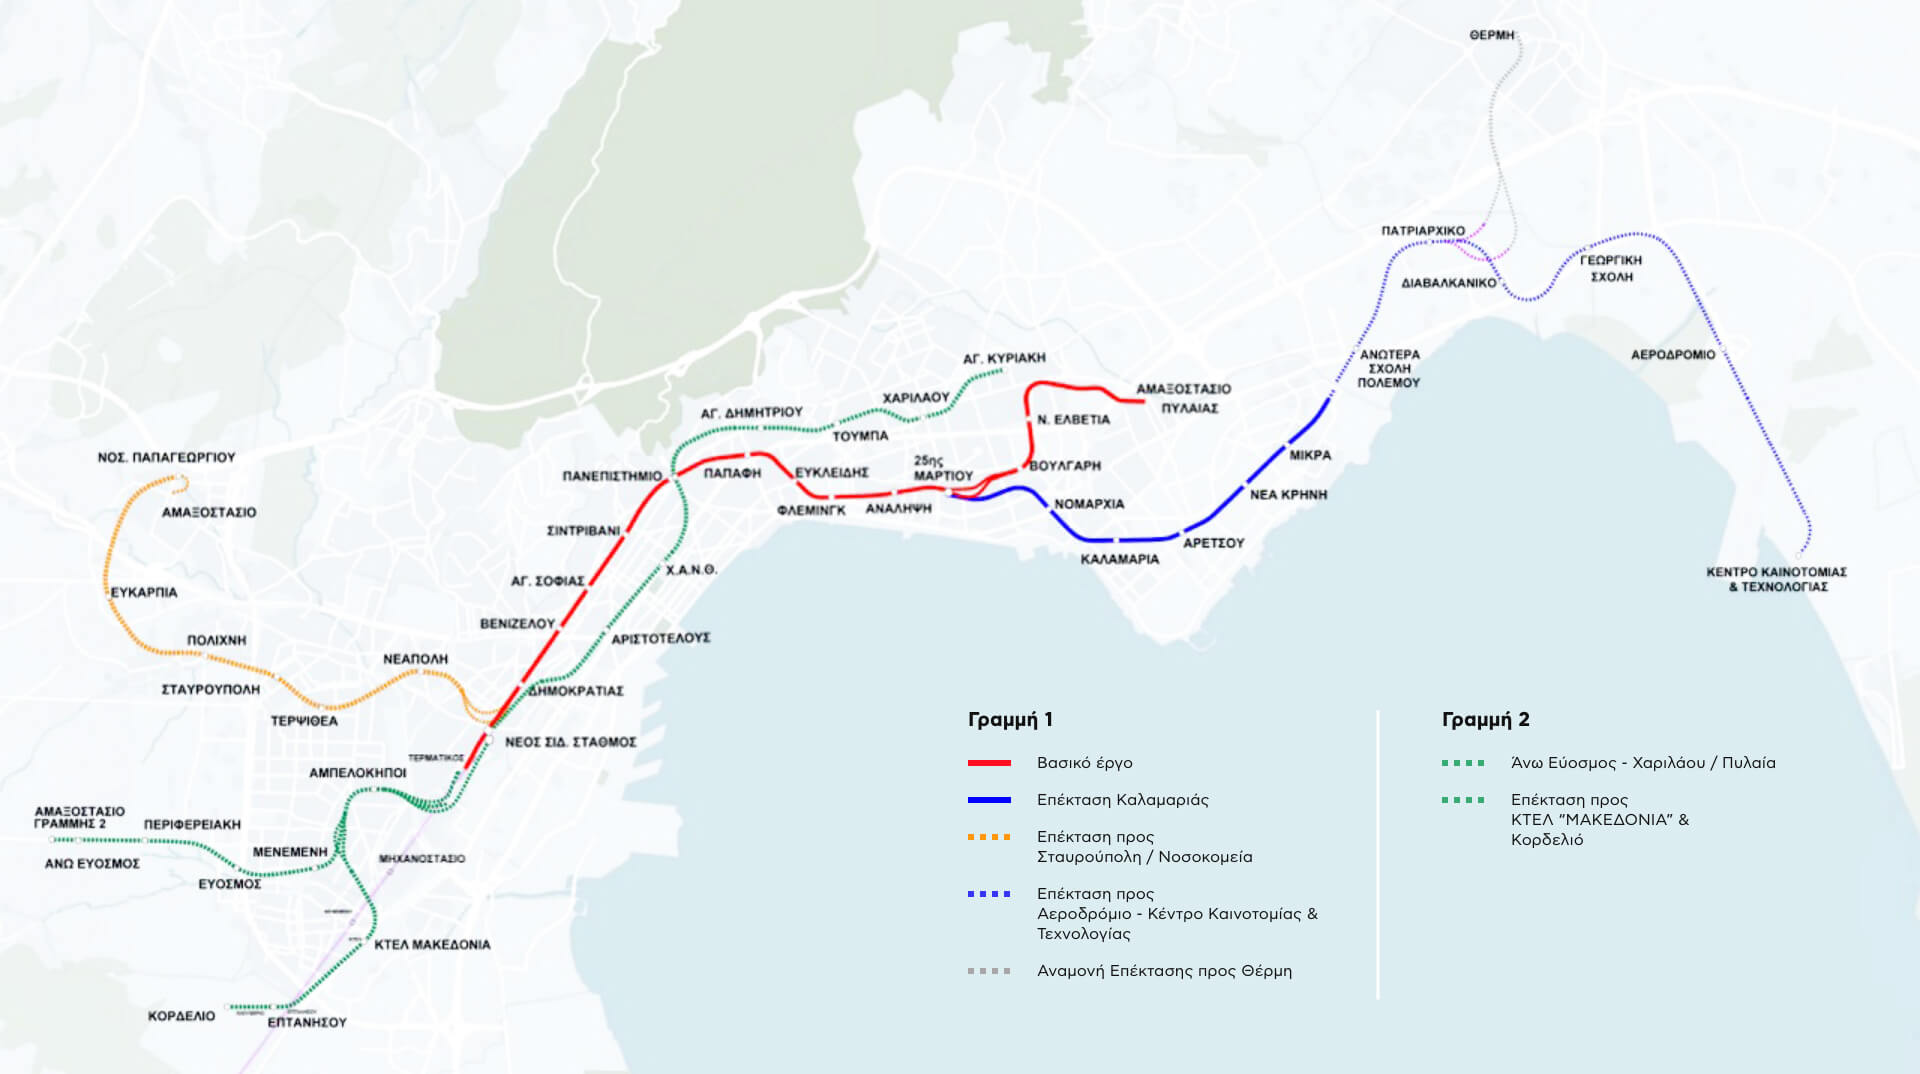
\includegraphics[width=0.95\linewidth]{figures/intro/Map.jpg}
	\label{fig:map}
	\caption{Το βασικό έργο και οι προβλεπόμενες επεκτάσεις (Πηγή: Ελληνικό Μετρό Α.Ε.)}
\end{figure}

Το μέλλον του μετρό Θεσσαλονίκης, όπως είναι η μοίρα των έργων υπογείων σηράγγων, είναι να επεκταθεί εκτενώς. Οι σχεδιασμένες και προτεινόμενες διαδρομές απεικονίζονται στον χάρτη του Σχήματος \ref{fig:map} με την επέκταση προς Καλαμαριά της πρώτης γραμμής να ετοιμάζεται για παράδοση ενόσω συγγράφεται το παρόν έργο, με πέντε νέους σταθμούς.

Στην συνέχεια, υπάρχουν τρεις κύριες επεκτάσεις που μελετώνται. Η μία είναι η περαιτέρω επέκταση από τον σταθμό της Μίκρας έως το αεροδρόμιο Μακεδονία, συσκεπάζοντας τις ανάγκες μετακίνησης των αεροπιβατών από και προς το κέντρο της πόλης με μετρό.

Παράλληλα, υπάρχει πρόταση επέκτασης της γραμμής 1 πέρα από τον τερματικό σταθμό του Νέου Σιδηροδρομικού Σταθμού έως την Σταυρούπολη, εξυπηρετόντας ένα σχετικά απομακρυσμένο μέρος της πόλης.

Ως προς τις αμεσότερα υλοποιήσιμες επεκτάσεις, έχει προταθεί η κατασκευή μίας δεύτερης γραμμής του μετρό, το οποίο να διανύει την πόλη εγγύτερα του παραλιακού μετώπου, και εκτεινόμενης έως τον Εύοσμο και το Κορδελιό, αλλά και συνδέοντας τον κεντρικό σταθμό υπεραστικών λεωφορείων με το δίκτυο του μετρό, μία σύνδεση που θα ευνοούσε ιδιαιτέρως την πόλη.
